\chapter{Análisis Estadístico Descriptivo}
\label{ch:descriptivo}

Previo a la inferencia econométrica causal desarrollada en el Capítulo \ref{ch:resultados}, este capítulo describe la fuente, la construcción, el comportamiento tendencial, la dispersión y las propiedades de integración de las series de tiempo argentinas, constituyendo la base empírica sobre la cual se fundamenta la estimación paramétrica de la Función de Reacción Fiscal. Como se detalla en la Sección \ref{sec:matriz_operacional} del Capítulo \ref{ch:metodologia}, la investigación trabaja con una ventana muestral única, 1996T1--2025T4 ($n=120$, treinta años exactos), construida mediante el empalme documentado en la Sección \ref{sec:empalme} de ese capítulo: sobre ella se calculan los estadísticos descriptivos, las propiedades de integración y la totalidad del protocolo de robustez de este capítulo, salvo indicación contraria. El tramo 2004T1--2025T4 ($n=88$), íntegramente de fuente primaria y sin ningún tramo empalmado, se conserva únicamente como sub-muestra de referencia de cobertura 100\,\% real dentro de esa ventana única (Sección \ref{sec:matriz_operacional} del Capítulo \ref{ch:metodologia}), y no como una segunda ventana de estimación; sus propiedades de integración, junto con las de la ventana completa, se reportan en la Sección \ref{sec:estacionariedad_ampliada} de este capítulo.

\section{Propiedades Estadísticas de la Muestra y Análisis Descriptivo}
\label{sec:propiedades_muestra}

Como paso preliminar a cualquier caracterización sustantiva de las series, corresponde examinar sus propiedades distribucionales agregadas, en particular el grado de apartamiento respecto de la normalidad, dado que dicho apartamiento condiciona la elección posterior entre técnicas de inferencia lineal convencionales y técnicas robustas a la asimetría y a la curtosis extrema (Sección \ref{sec:hansen} y Capítulo \ref{ch:discusion}). Este diagnóstico se computa sobre la sub-muestra de cobertura 100\,\% real (2004T1--2025T4, $n=88$) dentro de la ventana única (Sección \ref{sec:matriz_operacional} del Capítulo \ref{ch:metodologia}), para evitar mezclar en un mismo estadístico el tramo de fuente primaria directa con el tramo empalmado 1996--2003.

\begin{table}[H]
\centering
\caption{\label{tab:descriptivos_jb} Estadísticas descriptivas de los vectores empíricos agregados (2004--2025, n=88).}
\resizebox{\textwidth}{!}{%
\begin{tabular}{lrrrrrrr}
\toprule
\textbf{Variable} & \textbf{Media} & \textbf{Mediana} & \textbf{Desv. Est.} & \textbf{Mín.} & \textbf{Máx.} & \textbf{Jarque-Bera} & \textbf{$p$-valor (JB)} \\
\midrule
$pb_t$ (Result. Primario/PIB, \%) & -0.70 & -0.80 & 1.59 & -3.80 & 1.80 & 5.87 & 0.053 \\
$d_t$ (Deuda/PIB, \%) & 65.93 & 63.00 & 18.68 & 40.00 & 119.00 & 5.64 & 0.060 \\
$risk_t$ (EMBI+, pb) & 1298.21 & 808.80 & 1229.50 & 210.22 & 5626.29 & 128.58 & 0.00000 \\
$\tilde{y}_t$ (Brecha del Producto, \%) & -0.02 & -0.80 & 5.54 & -11.15 & 13.86 & 4.89 & 0.087 \\
\bottomrule
\end{tabular}%
}
\begin{flushleft}
\footnotesize \textit{Nota.} Elaboración propia en base a \texttt{dataset\_consolidado\_real.csv}. Estadístico de Jarque-Bera bajo hipótesis nula de normalidad.
\end{flushleft}
\end{table}

El contraste de Jarque-Bera exige una lectura diferenciada. El EMBI+ rechaza con contundencia la hipótesis nula de normalidad ($JB=128.58$, $p<0.00001$), resultado esperable dada su naturaleza de cola derecha extrema: los episodios de pánico financiero desplazan el indicador muy por encima de su media, y con la serie real ese rechazo es aún más categórico que el que arrojaba la serie de contingencia utilizada hasta la Sección \ref{sec:auditoria_fallback} del Capítulo \ref{ch:metodologia} ($JB=20.71$, $p=0.00003$). Las tres series restantes ($pb_t$, $d_t$ y $\tilde{y}_t$) exhiben $p$-valores marginales (0.05--0.09) que no permiten un rechazo al 5\% pero tampoco confirman normalidad, ubicándose en una zona de ambigüedad estadística coherente con muestras de tamaño moderado ($n=88$). Esta evidencia respalda la motivación metodológica para las técnicas robustas a la asimetría adoptadas en los capítulos subsiguientes: la regresión de umbral asimétrica de Hansen (Sección \ref{sec:hansen}) y el DSA estocástico no gaussiano (Capítulo \ref{ch:discusion}).

\section{Fuente, Cobertura y Construcción de la Matriz de Datos}

El panel trimestral comprende la ventana única de 120 observaciones (1996T1--2025T4, Sección \ref{sec:matriz_operacional} del Capítulo \ref{ch:metodologia}), integrando ocho variables construidas a partir de fuentes secundarias oficiales: el VIX, el EMBI+ argentino\footnote{Diferencial de rendimiento, ponderado por duración, entre bonos soberanos en dólares y Treasuries de EE.UU. comparables (J.P. Morgan).}, el CER, el TCRM, el PIB real, el Resultado Primario del SPNF (\% PIB), la Deuda Pública del SPNF (\% PIB) y la brecha del producto derivada mediante filtro Hodrick-Prescott ($\lambda=1600$). De estas ocho, seis (EMBI+, TCRM, PIB real, Resultado Primario, Deuda Pública y la brecha del producto derivada de esta última) cubren la ventana completa mediante el empalme documentado en la Sección \ref{sec:empalme} del Capítulo \ref{ch:metodologia}, y el VIX se extendió con serie real completa desde 1990; el CER, en cambio, no tiene existencia previa a febrero de 2002 y permanece confinado a su cobertura real de 2004T1--2025T4 (88 observaciones).

Sobre esta última variable corresponde una precisión metodológica. La literatura reciente \citep{hamilton2018} cuestiona el filtro HP en series macroeconómicas, señalando la introducción de ciclos espurios y distorsión sistemática en los extremos de la muestra. No obstante, esta investigación adopta $\lambda=1600$ por criterio de parsimonia y comparabilidad internacional con los manuales DSA del FMI y el BID, que emplean sistemáticamente esta convención. Como chequeo de robustez, se recalculó la brecha mediante el filtro de \citet{hamilton2018} ($h=8$, $p=4$ rezagos): ambas series presentan una correlación de $r=0.72$, un grado de acuerdo sustancial que sugiere que las conclusiones de la tesis no dependen críticamente de esta elección de diseño, aunque la correlación, lejos de la unidad, confirma que ambos métodos no son intercambiables.

La construcción de la matriz siguió un protocolo en dos etapas, detallado en el libro de códigos: obtención de datos desde las APIs de \url{apis.datos.gob.ar}, BCRA y Yahoo Finance, recurriendo a informes alternativos (CEPAL, FMI, JP Morgan, MECON) ante discontinuidades. La deuda pública incorporada en la especificación central corresponde a la deuda bruta del SPNF neta de tenencias intra-sector público (acreencias del FGS de la ANSES), corrección que reduce el ratio bruto publicado habitualmente en prensa entre 15 y 20 puntos porcentuales del PIB según el año, y resulta metodológicamente indispensable para evitar sobreestimar la exposición neta del Tesoro frente a acreedores extra-estatales.

\section{La Ventana Única: Descriptivos e Integración (1996--2025, n=120)}
\label{sec:ventana_ampliada}

El procedimiento de empalme descrito en la Sección \ref{sec:empalme} del Capítulo \ref{ch:metodologia} construye las cuatro variables del sistema de cointegración (deuda/PIB, resultado primario/PIB, EMBI+ y TCRM) sobre la ventana única de 120 observaciones trimestrales (1996T1--2025T4), de las cuales 32 (1996T1--2003T4) provienen del empalme y 88 (2004T1--2025T4) de fuente primaria directa, sin ningún tramo empalmado. La Tabla \ref{tab:descriptivos_ampliado} resume sus estadísticos sobre la ventana completa.

\begin{table}[H]
\centering
\caption{\label{tab:descriptivos_ampliado} Estadísticos descriptivos de las variables del sistema VECM (1996T1--2025T4, n=120).}
\begin{tabular}{lrrrrr}
\toprule
\textbf{Variable} & \textbf{Media} & \textbf{Desv. Est.} & \textbf{Mín.} & \textbf{Máx.} & \textbf{Asimetría} \\
\midrule
Deuda SPNF / PIB (\%) & 64.46 & 27.60 & 26.96 & 157.27 & 1.12 \\
Resultado Primario / PIB (\%) & -0.27 & 1.73 & -3.80 & 4.08 & 0.13 \\
EMBI+ (puntos básicos) & 1483.95 & 1573.84 & 210.22 & 6658.98 & 1.93 \\
TCRM (índice) & 1.63 & 0.45 & 0.98 & 2.76 & 0.52 \\
Brecha del Producto (\%) & -0.06 & 5.51 & -11.77 & 14.53 & 0.34 \\
\bottomrule
\end{tabular}
\begin{flushleft}
\footnotesize \textit{Nota.} Elaboración propia en base a \texttt{dataset\_consolidado\_1996\_2025.csv} (\texttt{codigo/modelos/fase23\_reestimacion\_1996\_2025.py}).
\end{flushleft}
\end{table}

Frente a la sub-muestra de cobertura 100\,\% real (Tabla \ref{tab:descriptivos}), la incorporación del tramo empalmado 1996--2003 desplaza sensiblemente los extremos: el mínimo de la deuda/PIB baja de 40.00\% a 26.96\% (el piso de la salida de la crisis, no capturado por esa sub-muestra, que arranca ya en el proceso de descompresión posterior al canje) y su máximo sube de 119.00\% a 157.27\% (el pico de la cesación de pagos de 2002, previo a la quita de 2005). El EMBI+ se desplaza en el mismo sentido pero de forma menos mecánica: su media sube de 1298 a 1484 puntos básicos, ya que la crisis de 2001--2002 empuja el promedio hacia arriba, como es esperable, y su asimetría se acentúa levemente (2.16 a 1.93): al incorporar además 1996--1998, con niveles de riesgo soberano moderados propios de la Convertibilidad, la cola derecha vuelve a alargarse en relación con un cuerpo de distribución más bajo. Estos desplazamientos no son un artefacto del empalme: reflejan la incorporación sustantiva de quiebres estructurales extremos (crisis del Tequila y colapso de la Convertibilidad) necesarios para evaluar la sostenibilidad fiscal a lo largo de un ciclo secular completo.

\subsection{Estacionariedad sobre la Ventana Única}
\label{sec:estacionariedad_ampliada}

La Tabla \ref{tab:estacionariedad_ampliado} repite el protocolo ADF/KPSS de la Sección \ref{sec:estacionariedad} sobre la ventana única, para las cuatro variables del sistema de cointegración y la brecha del producto.

\begin{table}[H]
\centering
\caption{\label{tab:estacionariedad_ampliado} Pruebas de raíz unitaria e integración, ventana única (1996T1--2025T4, n=120).}
\begin{tabular}{lccccc}
\toprule
\textbf{Variable} & \textbf{ADF $p$ (nivel)} & \textbf{KPSS $p$ (nivel)} & \textbf{ADF $p$ (dif.)} & \textbf{KPSS $p$ (dif.)} & \textbf{Orden} \\
\midrule
Deuda / PIB & 0.042 & 0.100 & 0.001 & 0.100 & I(1)$^{\dagger}$ \\
Result. Primario / PIB & 0.605 & 0.010 & 0.000 & 0.100 & I(1) \\
EMBI+ & 0.150 & 0.100 & 0.000 & 0.100 & I(1) \\
TCRM & 0.259 & 0.100 & 0.000 & 0.100 & I(1) \\
Brecha del Producto & 0.001 & 0.100 & 0.000 & 0.100 & I(0) \\
\bottomrule
\end{tabular}
\begin{flushleft}
\footnotesize \textit{Nota.} Elaboración propia en base a \texttt{dataset\_consolidado\_1996\_2025.csv} (\texttt{codigo/modelos/fase23\_reestimacion\_1996\_2025.py}). Test ADF bajo hipótesis nula de raíz unitaria; test KPSS bajo hipótesis nula de estacionariedad. $^{\dagger}$Ver discusión: el ADF rechaza la raíz unitaria al 5\%, un diagnóstico que por sí solo sugeriría I(0), no I(1).
\end{flushleft}
\end{table}

El resultado ya no es tan ordenado como en una iteración previa de esta investigación que empleaba una ventana ampliada de 108 observaciones (1999--2025), hoy superada. El resultado primario, el EMBI+ y el TCRM se mantienen I(1) sin ambigüedad, y la brecha del producto I(0), igual que antes. La deuda/PIB, en cambio, presenta un diagnóstico que se mueve en la dirección opuesta a la que traía esa ventana anterior: allí el ADF no rechazaba la raíz unitaria ($p=0.118$) y el KPSS quedaba en el límite superior tabulado, concluyéndose I(1). En la ventana de treinta años, el ADF sí rechaza la raíz unitaria al 5\% ($p=0.042$), lo que por sí solo apuntaría a I(0); pero el KPSS en niveles tampoco rechaza estacionariedad ($p=0.100$), de modo que ambos contrastes, leídos de forma aislada, favorecerían I(0) y no I(1). Esta tesis mantiene, no obstante, el tratamiento I(1) de la deuda/PIB para la estimación VECM/SVAR de la Sección \ref{sec:etapa2_johansen} del Capítulo \ref{ch:metodologia}, por dos motivos: primero, KPSS al límite tabulado del 10\% es una no-rechazo débil, no una confirmación robusta de estacionariedad; segundo, es la lectura que preserva la comparabilidad con el resto del protocolo y con el diagnóstico obtenido sobre la sub-muestra de cobertura 100\,\% real (Sección \ref{sec:estacionariedad}), donde la deuda/PIB también se trata como I(1) pese a un diagnóstico igualmente no concluyente. El contraste DF-GLS de \textcite{elliott1996}, de mayor potencia estadística y aplicado sobre esta misma ventana única en la Sección \ref{sec:dfgls} del Capítulo \ref{ch:resultados}, refuerza esta decisión: a diferencia del ADF simple, no rechaza la raíz unitaria en niveles para la deuda/PIB ($-2.65$ frente a un crítico de $-3.01$), respaldando con más autoridad el tratamiento I(1) adoptado aquí por criterio teórico. Se deja declarado que este es un punto de tensión genuino, no resuelto por el protocolo actual, y coherente con el resto de los hallazgos de esta ventana (Secciones \ref{sec:resultados_vecm} y \ref{sec:svar_resultados} del Capítulo \ref{ch:resultados}): una deuda/PIB con un componente de reversión a la media más marcado que antes es consistente tanto con la mayor dificultad para hallar cointegración de largo plazo como con el peso creciente de la inercia propia en la descomposición de varianza del SVAR.

\section{Distribución y Volatilidad de las Variables Base}

La Tabla \ref{tab:descriptivos} sintetiza los estadísticos descriptivos univariados de las siete variables continuas de la matriz de datos, sobre la sub-muestra de cobertura 100\,\% real (2004T1--2025T4, $n=88$): a diferencia de las cuatro variables del sistema de cointegración, reportadas sobre la ventana única completa en la Sección \ref{sec:ventana_ampliada}, el CER carece de cobertura anterior a 2004 (Sección \ref{sec:empalme} del Capítulo \ref{ch:metodologia}) y fija, por comparabilidad dentro de una misma tabla, la ventana de las siete variables aquí reportadas.

\begin{table}[H]
\centering
\caption{\label{tab:descriptivos} Estadísticos descriptivos de las variables macro-fiscales (2004T1--2025T4, n=88).}
\begin{tabular}{lrrrrr}
\toprule
\textbf{Variable} & \textbf{Media} & \textbf{Desv. Est.} & \textbf{Mín.} & \textbf{Máx.} & \textbf{Asimetría} \\
\midrule
EMBI+ (puntos básicos) & 1298.21 & 1229.50 & 210.22 & 5626.29 & 2.16 \\
Deuda SPNF / PIB (\%) & 65.93 & 18.68 & 40.00 & 119.00 & 0.60 \\
Resultado Primario / PIB (\%) & -0.70 & 1.59 & -3.80 & 1.80 & -0.01 \\
TCRM (índice) & 1.71 & 0.39 & 1.14 & 2.41 & 0.48 \\
Brecha del Producto (\%) & -0.02 & 5.54 & -11.15 & 13.86 & 0.59 \\
CER (índice acumulado) & 58.01 & 145.79 & 1.46 & 654.29 & 3.06 \\
VIX (puntos) & 18.98 & 7.48 & 10.31 & 58.60 & 2.46 \\
\bottomrule
\end{tabular}
\begin{flushleft}
\footnotesize \textit{Nota.} Elaboración propia en base a \texttt{dataset\_consolidado\_real.csv} (BCRA, MECON, INDEC, JP Morgan, datos.gob.ar).
\end{flushleft}
\end{table}

Tres regularidades son relevantes. Primero, el EMBI+ opera en un orden de magnitud muy superior al de economías emergentes con grado de inversión crediticia, y su asimetría positiva pronunciada (2.16) confirma la cola derecha propia de los episodios de pánico financiero, frente a fases de compresión del diferencial de riesgo comparativamente más graduales. Segundo, el Resultado Primario exhibe media negativa y asimetría prácticamente nula, compatible con la hipótesis de reacción fiscal débil de $H_{1a}$, mientras que la Deuda/PIB muestra una asimetría moderada que refleja la persistencia de episodios de sobreendeudamiento por encima de la media. Tercero, la asimetría extrema del CER (3.06) no expresa volatilidad financiera, sino la consecuencia mecánica de tratarse de un índice acumulativo de inflación pasada no comparable en niveles entre regímenes monetarios sucesivos, propiedad que la Sección \ref{sec:estacionariedad} somete a contraste formal de integración.

\section{Evolución del Vector de Solvencia: Deuda y Superávit}

El análisis temporal cruzado del ratio Deuda/PIB y el Resultado Primario, presentado en la Figura \ref{fig:dinamica_stocks_flujos}, permite visualizar la inoperancia práctica del teorema lineal de Bohn en la economía argentina.

\begin{figure}[H]
\centering
\caption{Dinámica Macrofiscal Agregada e Hitos de Reestructuración Soberana}
\label{fig:dinamica_stocks_flujos}

\includegraphics[width=0.95\textwidth]{fig5_1_deuda_resultado_primario.png}
\par\vspace{2mm}
{\footnotesize\textit{Nota.} Promedios anuales del panel trimestral, con ejes duales (deuda: eje izquierdo; resultado primario: eje derecho) y delimitación de los cuatro regímenes macrofiscales sucesivos. Elaboración propia en base a \texttt{dataset\_consolidado\_real.csv} (\texttt{codigo/graficos/generacion\_graficos\_tesis.py}).}
\end{figure}

La lectura revela cuatro regímenes sucesivos. Entre 2004 y 2011, la ratio de endeudamiento colapsa desde 110\% hasta un piso de 41.50\%, impulsada por la quita del canje de 2005 y por superávits primarios sostenidos (1.10\%--1.65\% del PIB) financiados por términos de intercambio favorables. Entre 2012 y 2017, el resultado primario se deteriora de manera continua hasta un déficit de 3.00\% del PIB en 2016, mientras la ratio de deuda recupera terreno moderadamente (de 43.00\% a 64.75\%). El tercer régimen, 2018--2020, es el más abrupto: la crisis cambiaria de 2018, el acuerdo \textit{stand-by} con el FMI (cuya ejecución fue objeto de una auditoría posterior de la Auditoría General de la Nación \citep{agn2023}) y la pandemia empujan la deuda hasta 94.50\% del PIB en apenas dos años. Finalmente, entre 2021 y 2025, el resultado primario retorna a terreno superavitario (1.58\% en 2024, 0.98\% en 2025) y la ratio de deuda desciende hasta 71.50\% del PIB.

Ninguno de estos cuatro regímenes se explica exclusivamente por el esfuerzo fiscal corriente: la descompresión 2004--2011 combina quita nominal, crecimiento del denominador y términos de intercambio favorables con auge de materias primas; el salto 2018--2020 combina devaluación real, prima de riesgo creciente y contracción del producto. Esta observación constituye la motivación empírica directa para instrumentar el riesgo soberano en el Capítulo \ref{ch:resultados}.

\section{Efecto Hoja de Balance: Tipo de Cambio Real y Variación de Deuda}
\label{sec:hoja_balance}

Como advierte la literatura sobre economías bimonetarias \citep{sanches2019}, cuando una porción sustancial del pasivo público está denominada en moneda extranjera, una devaluación del tipo de cambio real dispara mecánicamente el numerador de la ratio Deuda/PIB, independientemente del resultado primario contemporáneo. La Figura \ref{fig:hoja_balance} contrasta el nivel anual del TCRM con la variación interanual de la ratio de deuda.

\begin{figure}[H]
\centering
\caption{Efecto Hoja de Balance: Tipo de Cambio Real vs. Variación Anual de Deuda}
\label{fig:hoja_balance}
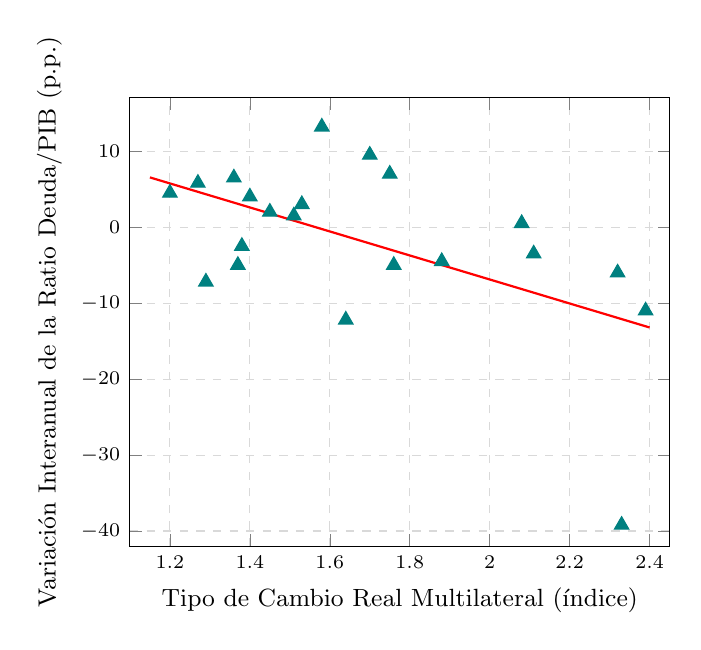
\begin{tikzpicture}
\begin{axis} [
    xlabel={Tipo de Cambio Real Multilateral (índice)},
    ylabel={Variación Interanual de la Ratio Deuda/PIB (p.p.)},
    xmin=1.10, xmax=2.45,
    ymin=-42, ymax=17,
    grid=both,
    grid style={dashed, gray!30},
    title style={font=\bfseries\small},
    label style={font=\small},
    tick label style={font=\scriptsize}
]
\addplot[only marks, mark=triangle*, color=teal, mark size=3pt] coordinates {
    (2.33,-39.2) (2.39,-11.0) (2.32,-6.0) (2.11,-3.5) (2.08,0.5) (1.88,-4.5)
    (1.76,-5.0) (1.51,1.5) (1.45,2.0) (1.53,3.0) (1.20,4.5) (1.36,6.5)
    (1.27,5.8) (1.58,13.2) (1.75,7.0) (1.70,9.5) (1.64,-12.2) (1.38,-2.5)
    (1.40,4.0) (1.37,-5.0) (1.29,-7.2)
};
\addplot[domain=1.15:2.4, red, thick] {-15.8*x + 24.71};
\end{axis}
\end{tikzpicture}
\par\vspace{2mm}
{\footnotesize\textit{Nota.} Impacto de las variaciones del tipo de cambio real sobre el stock de pasivos. Recta de ajuste MCO simple (referencial). Elaboración propia en base a \texttt{dataset\_consolidado\_real.csv} (BCRA, INDEC).}
\end{figure}

El primer punto (TCRM promedio 2005 $=2.33$, $\Delta d = -39.2$ p.p.) corresponde a la quita nominal del canje de deuda de 2005, no a un valor atípico de medición: se conserva en el gráfico por ser información genuina, y explica por sí solo buena parte de la pendiente negativa del ajuste MCO de nivel anual. Este resultado no debe confundirse con el mecanismo de hoja de balance propiamente dicho, que opera sobre \textit{variaciones} del tipo de cambio, no sobre su nivel. En términos de variaciones interperiódicas trimestrales, la correlación empírica entre la primera diferencia del TCRM ($\Delta TCRM_t$) y la variación de la ratio Deuda/PIB ($\Delta d_t$) alcanza $r=0.14$, positiva pero débil: consistente en signo con el mecanismo de hoja de balance, pero muy lejos de una relación determinística. Esta correlación es sensiblemente más débil que la calculada sobre el TCRM de contingencia utilizado hasta la Sección \ref{sec:auditoria_fallback} del Capítulo \ref{ch:metodologia} ($r=0.42$); la brecha ilustra cuánto podía distorsionar una relación bivariada simple el uso de una serie de contingencia suavizada en lugar de la serie real, y refuerza que la variación del endeudamiento obedece a una combinación de factores (resultado primario, crecimiento, tipo de cambio y ajustes stock-flujo), y no a un único indicador aislado.

\section{Protocolo de Estacionariedad y Pruebas de Raíz Unitaria}
\label{sec:estacionariedad}

Para evitar el riesgo de regresiones espurias, el protocolo evalúa el orden de integración de cada serie mediante dos contrastes complementarios: el test ADF (hipótesis nula: raíz unitaria) y el test KPSS (hipótesis nula: estacionariedad). La complementariedad de ambos, que testean hipótesis nulas opuestas, permite identificar con mayor robustez los casos ambiguos, especialmente relevantes en muestras de tamaño moderado como la sub-muestra de cobertura real aquí utilizada ($n=88$), necesaria para incluir al CER dentro de un panel comparable (Sección \ref{sec:empalme} del Capítulo \ref{ch:metodologia}).

\begin{table}[H]
\centering
\caption{\label{tab:estacionariedad} Pruebas de raíz unitaria e integración de las series (niveles y primeras diferencias).}
\resizebox{\textwidth}{!}{%
\begin{tabular}{lccccc}
\toprule
\textbf{Variable} & \textbf{ADF $p$ (nivel)} & \textbf{KPSS $p$ (nivel)} & \textbf{ADF $p$ (dif.)} & \textbf{KPSS $p$ (dif.)} & \textbf{Orden} \\
\midrule
Deuda / PIB & 0.113 & 0.041 & 0.000 & 0.035 & Ambiguo / I(1) \\
Result. Primario / PIB & 0.301 & 0.023 & 0.000 & 0.100 & I(1) \\
Brecha del Producto & 0.001 & 0.100 & 0.001 & 0.100 & I(0) \\
EMBI+ & 0.006 & 0.100 & 0.000 & 0.100 & I(0) \\
TCRM & 0.511 & 0.010 & 0.000 & 0.100 & I(1) \\
CER & 0.999 & 0.016 & 1.000 & 0.020 & Ambiguo / I(1) \\
\bottomrule
\end{tabular}%
}
\begin{flushleft}
\footnotesize \textit{Nota.} Elaboración propia. Test ADF bajo hipótesis nula de raíz unitaria; test KPSS bajo hipótesis nula de estacionariedad. p-valores reportados.
\end{flushleft}
\end{table}

Los resultados exhiben un panel de integración mixta, con implicancias metodológicas directas. La brecha del producto y el EMBI+ son estacionarias en niveles, I(0): oscilan en torno a una media constante, coherente con su naturaleza de variables cíclicas. El Resultado Primario y el TCRM son I(1): el ADF no rechaza la raíz unitaria en niveles mientras el KPSS rechaza estacionariedad; ambas se estabilizan tras la primera diferencia. Los casos de la Deuda/PIB y del CER producen un diagnóstico ambiguo, síntoma habitual de series estacionarias en torno a una tendencia con quiebre estructural (\textit{trend-stationary with a structural break}), que la Sección \ref{sec:zivot_andrews} somete a contraste formal.

Como evidencia visual complementaria, la Figura \ref{fig:acf_pacf} presenta los correlogramas ACF y PACF de las cuatro series núcleo. El decaimiento lento de la ACF del Resultado Primario y de la ratio Deuda/PIB, frente al corte abrupto tras el primer rezago de la Brecha del Producto y del EMBI+, ofrece una confirmación gráfica directa de la distinción entre series persistentes (I(1)) y de reversión rápida a la media (I(0)).

\begin{figure}[H]
\centering
\caption{Funciones de Autocorrelación Simple (ACF) y Parcial (PACF) de las Series Núcleo}
\label{fig:acf_pacf}

\includegraphics[width=0.85\textwidth]{figura_5_5_acf_pacf.png}
\par\vspace{2mm}
{\footnotesize\textit{Nota.} ACF (izquierda) y PACF (derecha, método Yule-Walker modificado) para 20 rezagos, con bandas de significatividad al 95\%. Elaboración propia en base a \texttt{dataset\_consolidado\_real.csv} (\texttt{codigo/modelos/fase7\_diagnosticos\_robustez.py}).}
\end{figure}

\subsection{Contraste de Zivot-Andrews con Quiebre Estructural Endógeno}
\label{sec:zivot_andrews}

A diferencia de los contrastes con quiebre exógeno (Chow, Perron), el algoritmo de Zivot-Andrews no requiere especificar \textit{a priori} la fecha de ruptura. El procedimiento itera sobre cada fecha candidata $T_B$ dentro de una ventana de recorte del 15\% en cada extremo, estimando para cada una la regresión MCO del Modelo C (quiebre simultáneo en intercepto y pendiente):
\[
\Delta d_t = c + \alpha\, d_{t-1} + \beta t + \theta\, DU_t(T_B) + \gamma\, DT_t(T_B) + \sum_{j=1}^{4} \phi_j \Delta d_{t-j} + \varepsilon_t
\]
donde $DU_t(T_B)=\mathbb{I}(t>T_B)$ y $DT_t(T_B)=(t-T_B)\cdot\mathbb{I}(t>T_B)$, y selecciona el $T_B$ que minimiza el estadístico $t$ asociado a $\alpha$. El rezago aumentado se fijó en $k=4$ trimestres.

Aplicado a la ratio Deuda/PIB sobre la ventana única (1996T1--2025T4, $n=120$), el algoritmo localiza el quiebre óptimo en 2004T2. El estadístico $t$ obtenido ($-4.50$) tampoco rechaza la hipótesis nula de raíz unitaria bajo ningún umbral crítico asintótico del Modelo C ($-5.58$ al 1\%, $-5.07$ al 5\%, $-4.83$ al 10\%), aunque se acerca sensiblemente más al crítico del 10\% que el resultado obtenido en una estimación previa sobre la sub-muestra de 88 observaciones ($t=-2.83$, quiebre en 2018T2). La ratio de deuda argentina se comporta, en consecuencia, como una serie genuinamente integrada de orden uno incluso permitiendo el quiebre más favorable a la alternativa de estacionariedad dentro de los treinta años de muestra. La restricción de un único quiebre es, además, insuficiente para una serie atravesada por múltiples reestructuraciones (2005, 2010, 2020) y episodios de interrupción repentina de capitales (\textit{sudden stop}, 2018), a los que ahora se suma la propia crisis de 2001--2002 dentro de la ventana: la Sección \ref{sec:quiebres_estructurales} extiende el análisis a un marco de quiebres múltiples, y la implicancia metodológica inmediata motiva la batería de pruebas de Johansen y la estimación DOLS desarrolladas en el Capítulo \ref{ch:resultados}.

\subsection{Deuda Consolidada: Incorporación de los Pasivos Remunerados del BCRA}
\label{sec:deuda_consolidada}

La delimitación del Capítulo \ref{ch:metodologia} circunscribe $d_t$ al SPNF, excluyendo la absorción monetaria del BCRA: LEBAC/NOBAC (2002--2018), LELIQ/NOTALIQ (2018--2024) y la posición neta de pases. El devengamiento de intereses de estos instrumentos constituye un déficit cuasi-fiscal ausente del resultado primario del Tesoro, estimado en el orden del 9\%--10\% del PIB en su pico reciente. Como extensión de robustez, se construyó una serie de pasivos remunerados del BCRA a partir de las series oficiales v4.0 del BCRA (idVariable 1258, 1260 y 1261) y del PIB nominal trimestral de INDEC, sin neteo adicional entre ambos stocks.

La brecha promedio entre ambas definiciones es de 5.5 puntos porcentuales del PIB, con un pico de 10.6\% en el primer trimestre de 2018 y una caída a valores prácticamente nulos desde mediados de 2024, cuando el Tesoro asumió el rol de esterilizador monetario mediante Letras Fiscales de Liquidez (LEFI). La Figura \ref{fig:deuda_consolidada} contrasta ambas series.

\begin{figure}[H]
\centering
\caption{Deuda Pública: SPNF vs. Consolidada con Pasivos Remunerados del BCRA}
\label{fig:deuda_consolidada}

\includegraphics[width=0.95\textwidth]{figura_8_1_deuda_consolidada.png}
\par\vspace{2mm}
{\footnotesize\textit{Nota.} Elaboración propia en base a series oficiales BCRA v4.0 y PIB nominal INDEC (\texttt{codigo/ingesta\_datos/ingesta\_bcra\_pasivos.py}, \texttt{codigo/modelos/fase8\_deuda\_consolidada.py}).}
\end{figure}

La serie consolidada conserva el orden de integración de la serie SPNF (ADF no rechaza en niveles, $p=0.169$; rechaza en primera diferencia, $p<0.001$; KPSS rechaza estacionariedad en niveles, $p=0.038$), coherente con I(1). La Sección \ref{sec:quiebres_estructurales} evalúa si la cronología de quiebres estructurales se modifica al incorporar esta capa cuasi-fiscal.

\subsection{Quiebres Estructurales Múltiples de Bai-Perron}
\label{sec:quiebres_estructurales}

El test de Zivot-Andrews impone la restricción de un único quiebre, insuficiente para una serie atravesada por las reestructuraciones soberanas de 2005, 2010 y 2020 y los episodios de \textit{sudden stop}. \textcite{bai2003} resuelven esta limitación estimando de manera consistente el número y la ubicación de quiebres múltiples sin conocimiento \textit{a priori} de sus fechas, mediante programación dinámica sobre la suma de cuadrados residuales de las particiones factibles, con selección del número de quiebres por el criterio BIC \citep{yao1988}.

El criterio BIC selecciona $m^*=3$ quiebres para la deuda SPNF sobre la ventana única completa (1996T1--2025T4, $n=120$): 2001T3, 2006T1 y 2017T3. Las medias estimadas por segmento son 34.68\% (1996T1--2001T3, $n=23$), 106.85\% (2001T4--2006T1, $n=18$), 50.72\% (2006T2--2017T3, $n=46$) y 81.24\% (2017T4--2025T4, $n=33$) del PIB: al incorporar el tramo 1996--2003, el algoritmo detecta por primera vez el quiebre de la crisis de 2001, invisible para una ventana que arrancara en 2004. Para la deuda consolidada con pasivos del BCRA, cuya cobertura permanece acotada a la sub-muestra de fuente primaria real (2004T1--2025T4, $n=88$, Sección \ref{sec:deuda_consolidada}) por no existir una serie de pasivos remunerados del BCRA verificable antes de 2004, el criterio selecciona $m^*=2$ quiebres en 2007T2 y 2016T4, con medias de 81.8\%, 53.5\% y 86.4\%, una cronología distinta a la de la deuda SPNF sola, coherente con que el peso cuasi-fiscal del BCRA introduce su propia dinámica de régimen.

\begin{figure}[H]
\centering
\caption{Quiebres Estructurales Múltiples de Bai-Perron (Selección por BIC)}
\label{fig:bai_perron}

\includegraphics[width=0.95\textwidth]{figura_9_1_bai_perron.png}
\par\vspace{2mm}
{\footnotesize\textit{Nota.} Deuda SPNF vs. deuda consolidada SPNF+BCRA, con quiebres óptimos de Bai-Perron ($m^*=3$ y $m^*=2$ respectivamente) y medias de segmento superpuestas. Elaboración propia en base a \texttt{dataset\_consolidado\_real.csv} (\texttt{codigo/modelos/fase9\_bai\_perron.py}).}
\end{figure}

Como evidencia exploratoria complementaria, se aplicó sobre el Resultado Primario un algoritmo de detección de quiebres por programación dinámica de costo $L_2$ (paquete \texttt{ruptures} \citep{truong2020}), fijando cuatro particiones para permitir una lectura comparable con los cuatro regímenes macrofiscales de la Figura \ref{fig:dinamica_stocks_flujos}.

\begin{figure}[H]
\centering
\caption{Cronología de Quiebres Estructurales Múltiples en el Resultado Primario}
\label{fig:quiebres_timeline}

\includegraphics[width=0.95\textwidth]{figura_5_4_quiebres_timeline.png}
\par\vspace{2mm}
{\footnotesize\textit{Nota.} Quiebres detectados mediante programación dinámica (costo $L_2$, \texttt{ruptures}), en el espíritu del enfoque de partición óptima de \textcite{bai2003} (Sección \ref{sec:zivot_andrews}). Elaboración propia en base a \texttt{dataset\_consolidado\_real.csv} (\texttt{codigo/graficos/generacion\_cronologia\_quiebres.py}).}
\end{figure}

Los cuatro quiebres detectados (2008T3, 2013T2, 2019T1 y 2024T1) se aproximan a los límites de los cuatro regímenes macrofiscales identificados en la Sección anterior, con desfases de entre uno y cuatro trimestres. Esta coincidencia aproximada confirma que los regímenes macrofiscales identificados no son arbitrarios, aunque no coinciden mecánicamente con el punto de quiebre estadísticamente óptimo de la serie de resultado primario aislada.

\section{Matriz de Correlaciones Bivariadas y Diagnóstico de Multicolinealidad}
\label{sec:correlaciones_vif}

La evaluación de las correlaciones bivariadas arroja tres resultados relevantes para el diseño de la estrategia de instrumentación del Capítulo \ref{ch:resultados}. El VIX y el EMBI+ exhiben una correlación positiva pero prácticamente nula ($r=0.08$) en nivel contemporáneo: sobre la serie real de EMBI+, el canal de fuga hacia la calidad (vuelo hacia la calidad) de la literatura de finanzas internacionales no se manifiesta en la correlación simple de niveles, a diferencia de lo que sugería la serie de contingencia usada hasta la Sección \ref{sec:auditoria_fallback} del Capítulo \ref{ch:metodologia} ($r=0.33$); lo que no descarta el canal sino que exige una especificación menos ingenua (dinámica, no contemporánea) para detectarlo, motivo adicional para instrumentar el EMBI+ con el VIX en la Etapa 4 (Capítulo \ref{ch:resultados}) en lugar de inferir la relación de una correlación de nivel. La brecha del producto y el resultado primario muestran una correlación prácticamente nula ($r=0.07$). Esto no debe leerse como evidencia de una política contracíclica ejemplar: advierte, en cambio, que la correlación contemporánea simple no captura relaciones rezagadas, no lineales, ni mediadas por terceras variables, que la estimación multivariada del Capítulo \ref{ch:resultados} sí controla. Finalmente, la correlación entre la primera diferencia del TCRM y de la ratio de deuda ($r=0.14$, Sección \ref{sec:hoja_balance}) es positiva pero débil, la más débil de las tres pese a ser, sobre la serie de contingencia previa, la que se reportaba como más robusta.

La correlación bivariada, no obstante, no permite descartar dependencias lineales entre tres o más regresores simultáneamente. Se complementa por ello con los factores de inflación de la varianza (VIF) y el número de condición de la matriz de regresores estandarizados, calculados sobre las dos especificaciones relevantes para el Capítulo \ref{ch:resultados} y reportados en la Tabla \ref{tab:vif}.

\begin{table}[H]
\centering
\caption{\label{tab:vif} Diagnóstico de Multicolinealidad: Factores de Inflación de la Varianza y Número de Condición.}
\begin{tabular}{llrr}
\toprule
\textbf{Especificación} & \textbf{Regresor} & \textbf{VIF} & \textbf{Núm. de condición} \\
\midrule
\multirow{2}{*}{Núcleo de Bohn (DOLS)} & $d_{t-1}$ & 1.020 & \multirow{2}{*}{1.151} \\
 & Brecha del producto ($\tilde{y}_t$) & 1.020 & \\
\midrule
\multirow{4}{*}{Ampliada (Bohn + EMBI+ + TCRM)} & $d_{t-1}$ & 1.869 & \multirow{4}{*}{2.381} \\
 & Brecha del producto ($\tilde{y}_t$) & 1.025 & \\
 & EMBI+ & 1.910 & \\
 & TCRM & 1.046 & \\
\bottomrule
\end{tabular}
\begin{flushleft}
\footnotesize \textit{Nota.} $n=87$ en ambas especificaciones. Umbrales convencionales de alerta: $VIF>10$ y número de condición $>30$. El número de condición se computa sobre los regresores estandarizados, excluyendo la constante. Elaboración propia en base a \texttt{dataset\_consolidado\_real.csv} (\texttt{codigo/modelos/fase12\_diagnosticos\_complementarios.py}).
\end{flushleft}
\end{table}

Ninguna de las dos especificaciones exhibe multicolinealidad problemática. En el núcleo de Bohn, la especificación efectivamente estimada por DOLS, los dos regresores son prácticamente ortogonales ($VIF=1.02$, número de condición $=1.15$). En la especificación ampliada, con la serie real de TCRM y EMBI+, los cuatro regresores permanecen igualmente cerca de la ortogonalidad ($VIF$ entre $1.02$ y $1.91$, número de condición $=2.38$), muy por debajo tanto del umbral convencional de $10$ como del número de condición de $30$. Sobre la serie de contingencia utilizada hasta la Sección \ref{sec:auditoria_fallback} del Capítulo \ref{ch:metodologia}, el VIF de $d_{t-1}$ y de TCRM llegaba a $3.82$ y $3.69$ respectivamente (número de condición $3.84$): también por debajo de los umbrales de alerta, pero sensiblemente más alto que con la serie real, un indicio adicional de que la serie de contingencia introducía una colinealidad artificial con la trayectoria de la deuda que la serie real no reproduce. La imprecisión de los coeficientes reportada en el Capítulo \ref{ch:resultados} no es, en ningún caso, atribuible a colinealidad entre regresores.

\section{Dispersión Empírica y la Hipótesis de Fatiga Fiscal}

Como aproximación descriptiva preliminar a la hipótesis central de esta tesis ($H_{1a}$), la Figura \ref{fig:scatter_fatiga} cruza el nivel de deuda heredado ($d_{t-1}$) con el esfuerzo fiscal contemporáneo ($pb_t$) para el panel trimestral completo.

\begin{figure}[H]
\centering
\caption{Dispersión Empírica: Esfuerzo Primario vs. Endeudamiento Heredado}
\label{fig:scatter_fatiga}

\includegraphics[width=0.85\textwidth]{fig5_3_dispersion_fatiga_fiscal.png}
\par\vspace{2mm}
{\footnotesize\textit{Nota.} Dispersión empírica trimestral completa (87 pares $(d_{t-1}, pb_t)$), con ajuste polinómico local de segundo grado e intervalo de confianza del 95\% sombreado. Elaboración propia en base a \texttt{dataset\_consolidado\_real.csv} (\texttt{codigo/graficos/generacion\_graficos\_tesis.py}).}
\end{figure}

La nube de puntos sugiere, a simple vista, un patrón compatible con la hipótesis de fatiga fiscal: los superávits más altos (en torno a 1.00\%--1.60\% del PIB) se concentran en la región de deuda baja o moderada (40.00\%--70.00\%), mientras que la región de deuda elevada (80.00\%--120.00\%) exhibe mayoritariamente resultados deficitarios, con dos excepciones recientes (2024--2025) que reintroducen superávits modestos bajo un nivel de deuda todavía relativamente alto (79.00\% y 73.00\%). Es necesario, no obstante, evitar inferir un umbral en esta etapa descriptiva bivariada: la dispersión no controla por la brecha del producto, el riesgo soberano contemporáneo ni la dinámica temporal de la serie, todos ellos factores que la especificación de umbral formal de \citet{hansen1999} incorpora explícitamente en el Capítulo \ref{ch:resultados}. Como se mostrará allí, cuando estos controles se introducen, la evidencia estadística del quiebre sugerido visualmente pierde buena parte de su fuerza aparente en la especificación de nivel, aunque una especificación alternativa formalmente más apropiada la recupera (Sección \ref{sec:robustez_hansen_dpb}).

\section{Limitaciones de la Muestra y Advertencias de Inferencia}
\label{sec:limitaciones_muestra}

Los resultados presentados en este capítulo, y los que se desarrollarán en los Capítulos \ref{ch:resultados} y \ref{ch:discusion}, deben interpretarse a la luz de las limitaciones inherentes a la muestra. Las 120 observaciones trimestrales (1996T1--2025T4) constituyen la ventana muestral única de esta investigación (Sección \ref{sec:matriz_operacional} del Capítulo \ref{ch:metodologia}), de las cuales 88 (2004T1--2025T4) corresponden a la sub-muestra de cobertura 100\,\% real, sin tramo empalmado. Esta longitud muestral, adecuada para series de tiempo de un único país en condiciones de estacionariedad, limita la potencia estadística de pruebas como el umbral de Hansen y la cointegración de Johansen, especialmente en presencia de quiebres estructurales frecuentes.

El contexto de alta volatilidad estructural y regímenes de política cambiante, documentado en la cronología de Bai-Perron (Sección \ref{sec:quiebres_estructurales}), agrava esta limitación: cuando la variable de umbral (EMBI+, $\sigma=1573.84$ pb sobre la ventana única, Tabla \ref{tab:descriptivos_ampliado}) y la dependiente (resultado primario, $\sigma=1.73$ pp del PIB) están ambas sometidas a perturbaciones de magnitud comparable a la señal buscada, la relación señal-ruido se vuelve desfavorable para la identificación de quiebres discretos. Los tests de robustez implementados (subperíodos, especificaciones alternativas) confirman la fragilidad de inferencias fuertes sobre la significatividad estadística de los coeficientes individuales, lo que refuerza la necesidad de cautela en las proyecciones y de priorizar la consistencia del diagnóstico cualitativo sobre la precisión puntual de los estimadores.

La ventana única de 120 observaciones (Sección \ref{sec:ventana_ampliada}), que sostiene la totalidad del protocolo econométrico del Capítulo \ref{ch:resultados}, no releva de esta cautela: la desplaza a un terreno más nítido y, a la vez, más preocupante. El contraste de Johansen sobre la ventana 1996--2025 no rechaza la ausencia de cointegración para $r=0$ (traza $=45.18$ frente al valor crítico al 95\% de $47.85$), y el resultado se sostiene al variar el año de inicio de la muestra: la verificación sobre 1997--2025 ($n=116$, sin el empalme aproximado del TCRM de 1996) arroja una traza de $45.46$, prácticamente idéntica y también por debajo de ese mismo crítico. A diferencia de la ventana 1999--2025, que rechazaba $r=0$ en un punto de inicio de la muestra pero no en el otro, la ventana 1996--2025 no rechaza $r=0$ en ninguno de los dos puntos de inicio probados (Capítulo \ref{ch:resultados}): la ambigüedad sobre la existencia de una relación de cointegración estable no se reduce al ampliar la muestra, sino que se vuelve más marcada. Se impone $r=1$ por el mismo criterio teórico que ya empleaba la tesis, documentando explícitamente que esa imposición queda ahora menos respaldada por la evidencia estadística que antes.

Para abordar formalmente esta tensión entre longitud muestral y homogeneidad institucional, el Capítulo \ref{ch:resultados} (Sección \ref{sec:spread_historico_1983_2025}) desarrolla una extensión complementaria de ultra-largo plazo que reconstruye y empalma el spread soberano para los 42 años completos de democracia ininterrumpida ($1983\text{T4}$--$2025\text{T4}$, $n=169$), contrastando si los umbrales de fatiga fiscal identificados en la muestra central constituyen regularidades estructurales o artefactos circunscritos a las últimas dos décadas.

